\documentclass[12pt]{beamer}
\usepackage{mathtools}
\usepackage{makecell}
\usepackage{caption}
\captionsetup[figure]{labelformat=empty}
\useoutertheme{infolines}
\usetheme{default}
\usefonttheme{serif}
%\usefonttheme{structuresmallcapsserif}
\hypersetup{colorlinks=true,linkcolor=blue}
\setbeamertemplate{navigation symbols}{}
\setbeamertemplate{footline}[frame number]{}
\setbeamertemplate{footline}{}
\author{Mittereder, \textit{et. al.}}
\definecolor{darkgreen}{rgb}{0,.5,0}
\setlength{\parskip}{.1in}

\begin{document}

\begin{frame}[c]{} % Stephen

\begin{center}
\Large
The Impact of Social Network Density,\\Agent Openness, and Cross-Issue
Influence\\on Societal Polarization

\footnotesize
\vspace{.3in}
CSS 2021 --- Santa Fe, New Mexico (sorta)\\
\vspace{.1in}
\textbf{Justin Mittereder}, Robert Carroll, Brandon Frulla,
\textbf{Stephen Davies}\\
\scriptsize
\smallskip
Dept of Computer Science\\
University of Mary Washington\\
Fredericksburg, Virginia, USA\\
\bigskip
\bigskip
\texttt{https://github.com/jmittere/Peacemakers}
\end{center}

\end{frame}

\begin{frame}[c]{Defining polarization} % Stephen

\large

\centering
``America is becoming increasingly polarized..."

\vspace{-.2in}
\begin{figure}
\includegraphics[width=0.50\textwidth]{images/capitol.png}
\end{figure}
\pause
\vspace{-.2in}
What does this actually mean?
\vspace{-.15in}
\pause

\small
\begin{itemize}
\itemsep.1em
\item People's views becoming more \textit{extreme}?
\pause
\item People's dialogue becoming more \textit{combative}?
\pause
\item People becoming more \textit{stubborn}? (less willing to reconsider views)
\pause
\item People only associating with like-minded others? (echo chambers)
\end{itemize}

\end{frame}

\begin{frame}[c]{Polarization Proxy \#1: Assortativity coefficient} % Justin

% explain why we think this is a measure of polarization

% "Imagine if you had a social network, and each agent had an opinion on some
% issue that was between 0 and 1. You could think of it as liberal vs.
% conservative, perhaps."

% "echo chambers"
\small 	\textbf{Assortativity} measures the tendency of agents to associate with other like-minded agents. 
	\vspace{0.2in}
\begin{columns}[onlytextwidth]
\begin{column}{.50\textwidth}
\begin{figure}
	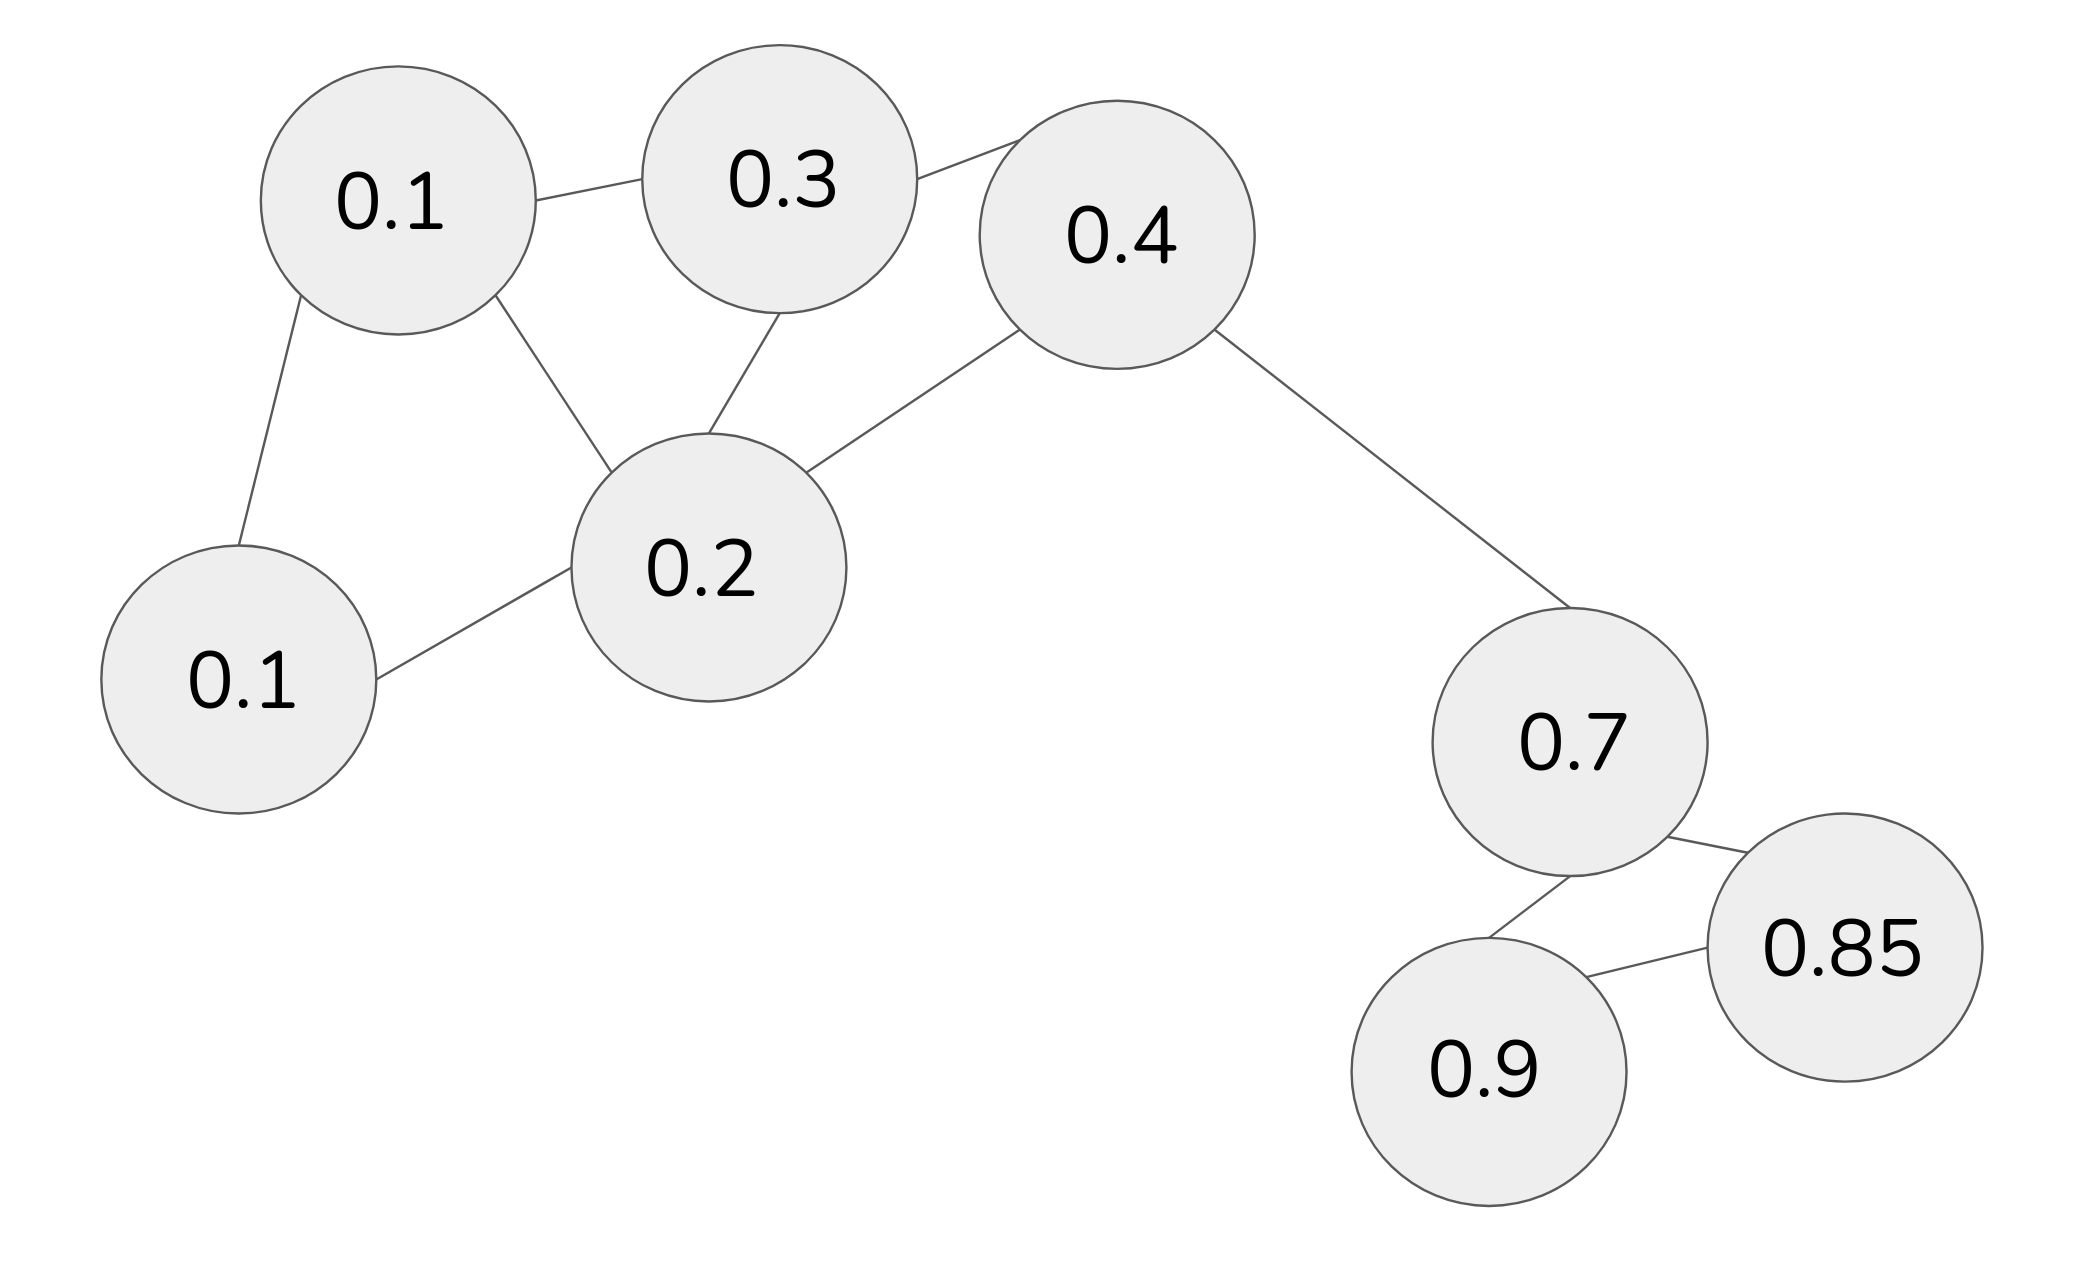
\includegraphics[width=0.90\textwidth]{images/HighAssortDiagram.png}
	\small \caption{High Assortativity}
\end{figure}
\end{column}
\hfill
\begin{column}{.50\textwidth}
\begin{figure}
	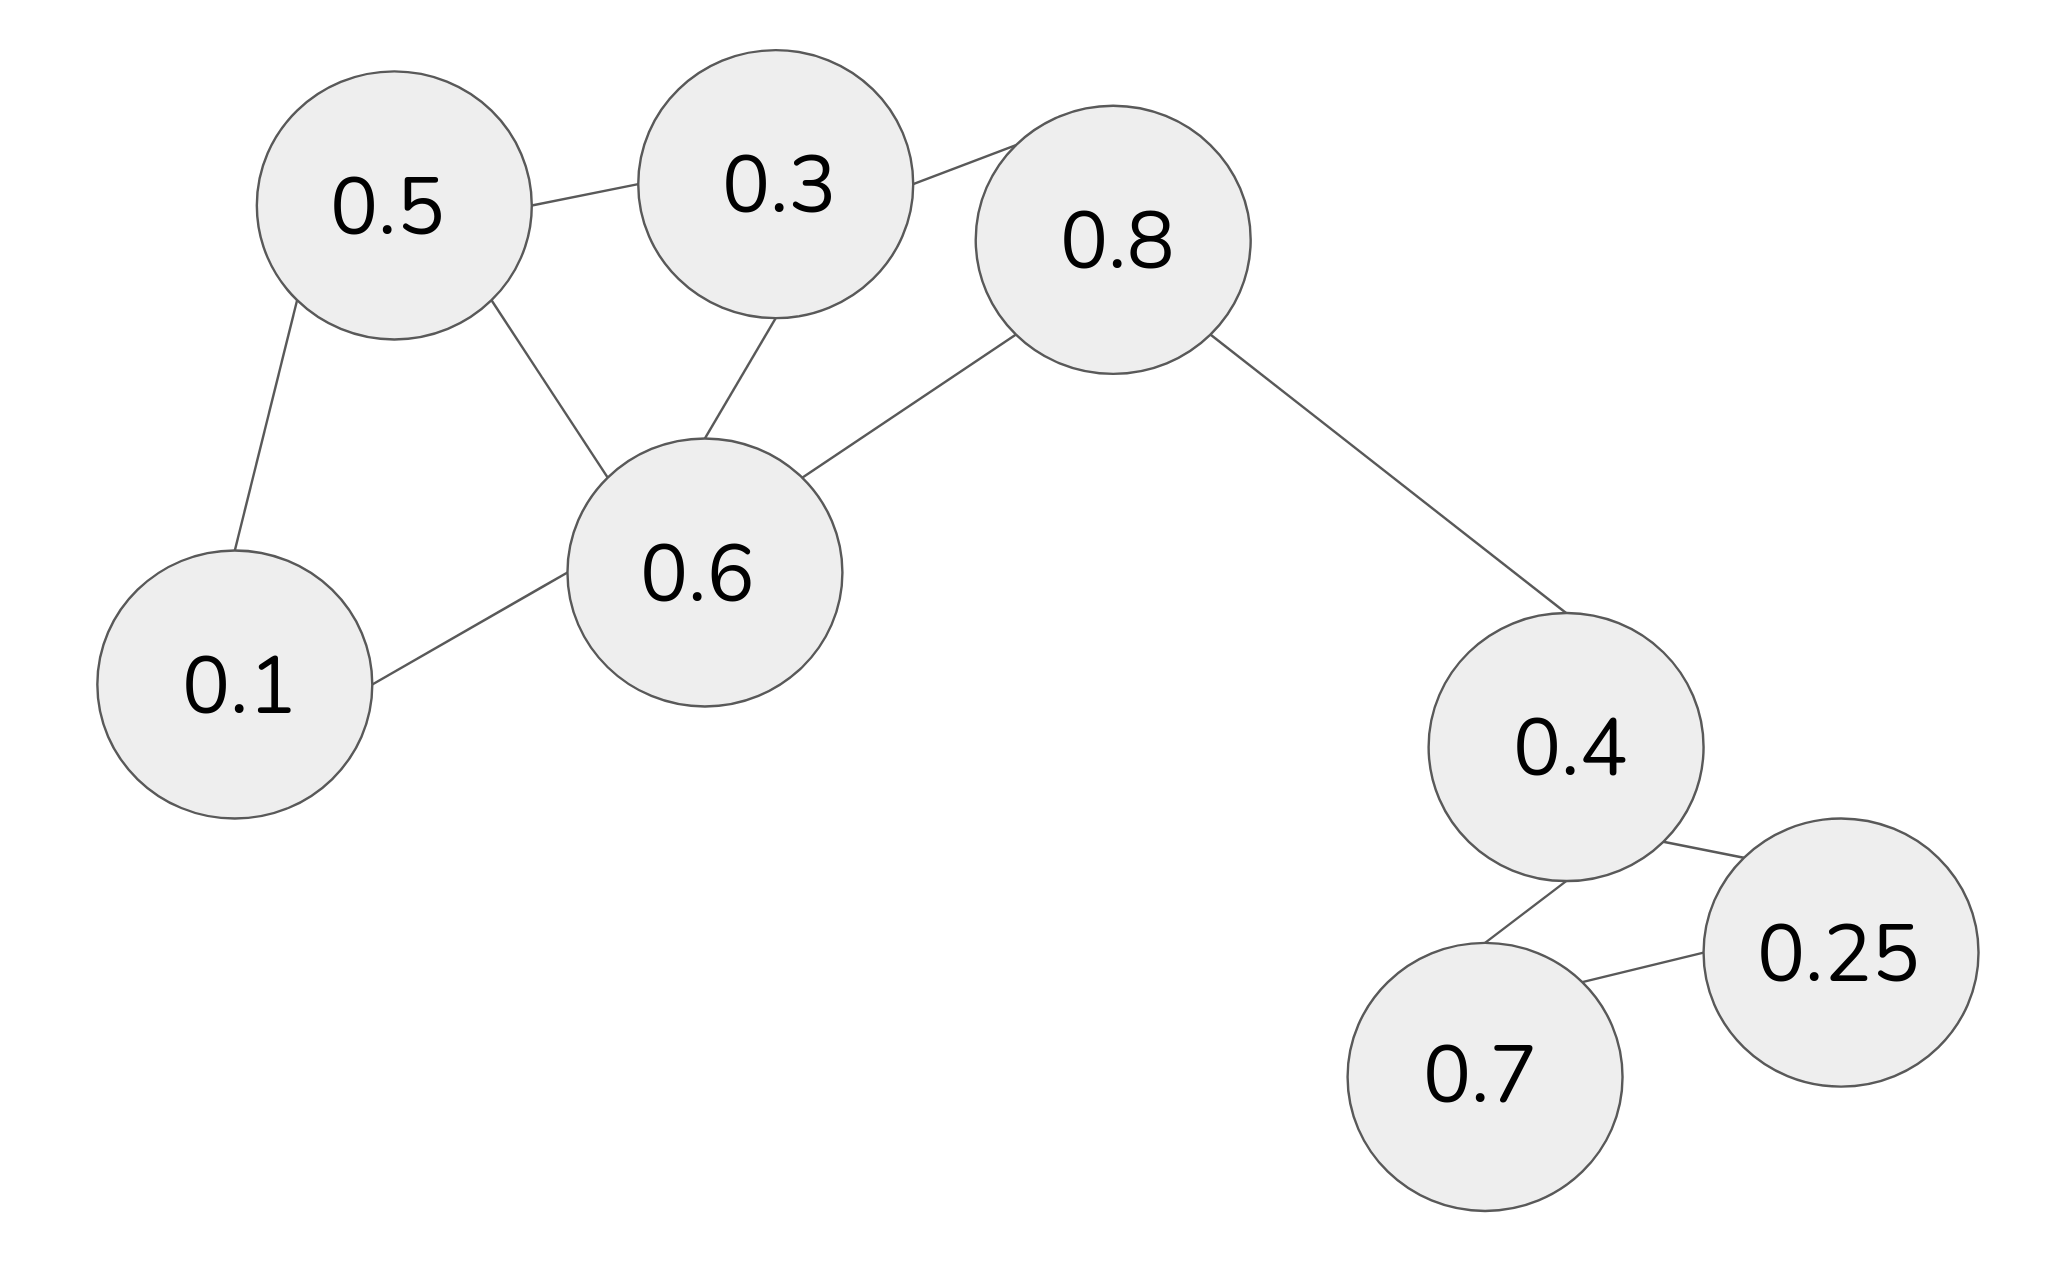
\includegraphics[width=0.90\textwidth]{images/LowAssortDiagram.png}
	\small \caption{Low Assortativity}
\end{figure}
\end{column}
\end{columns}

\end{frame}



\begin{frame}[c]{The model}  % Justin

% Describe in selected detail the model

% N heterogeneous agents who encounter each other on a social network.

% ER edge prob is a parameter

% Multiple continuous opinions 
\large

\centering
	\underline{Opinion Dynamics ABM with Mesa}

\vspace{.05in}
	Model Characteristics:
\vspace{-.15in}

\small
\begin{itemize}
\itemsep.1em
\item \textit{N} heterogenous agents who encounter each other on a social network.
\item \textbf{Edge Probability} of a random Erd\"{o}s-R\'{e}nyi graph which controls network density
\item Agents have opinions on multiple issues, each of which is on a continuum

% Slow down a bit on this last item: express with your voice that unlike the
% previous points, this is kind of a different thing than the audience might be
% used to.

\item \textbf{Openness Threshold} and \textbf{Disgust Threshold} that control the degree of agent opinion influence
\end{itemize}


\end{frame}


\begin{frame}[c]{\normalsize Traditional Bounded Confidence (Positive Influence)}  % Justin

% Here is traditional bounded confidence (BC) from Hegelsmen-Krause and
% Deffuant et al

% Take your time here, and explain who the blue guy is and who the grey guy is
% and what the 0-1 number line means.

\begin{figure}
	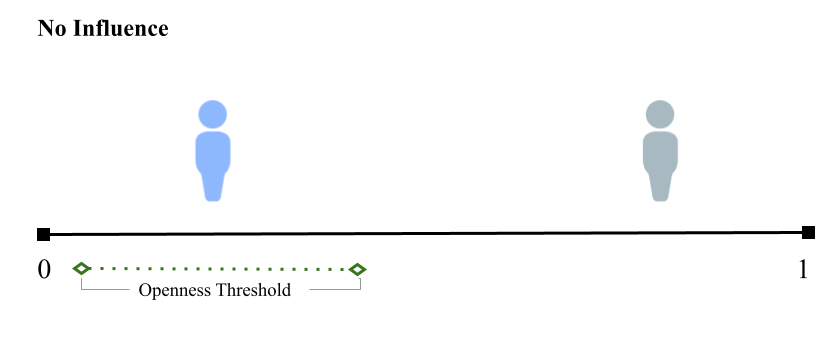
\includegraphics[width=0.65\textwidth]{images/BCNoInfluence.png}
	\hfill
	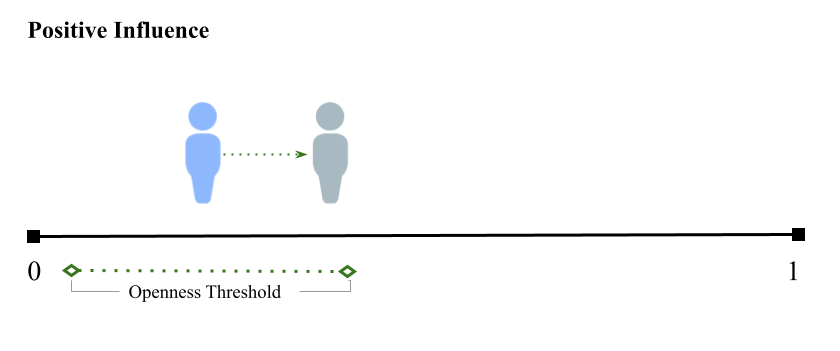
\includegraphics[width=0.65\textwidth]{images/BCPositiveInfluence.png}
\end{figure}


\end{frame}

\begin{frame}[c]{\normalsize Traditional Bounded Confidence (Negative Influence)}  % Justin

% Here is traditional bounded confidence (BC) from Hegelsmen-Krause/Deffuant with repulsion

\begin{figure}
	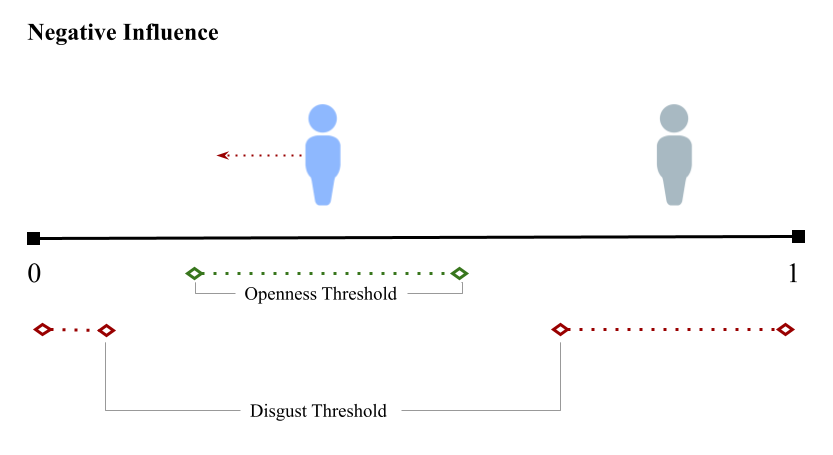
\includegraphics[width=0.65\textwidth]{images/BCNegativeInfluence.png}
\end{figure}


\end{frame}


\begin{frame}[c]{Results: Assortativity and Network Density}  % Justin

% Slow down, and make this point slower.
% Walk them through what the axes are.

\begin{figure}
	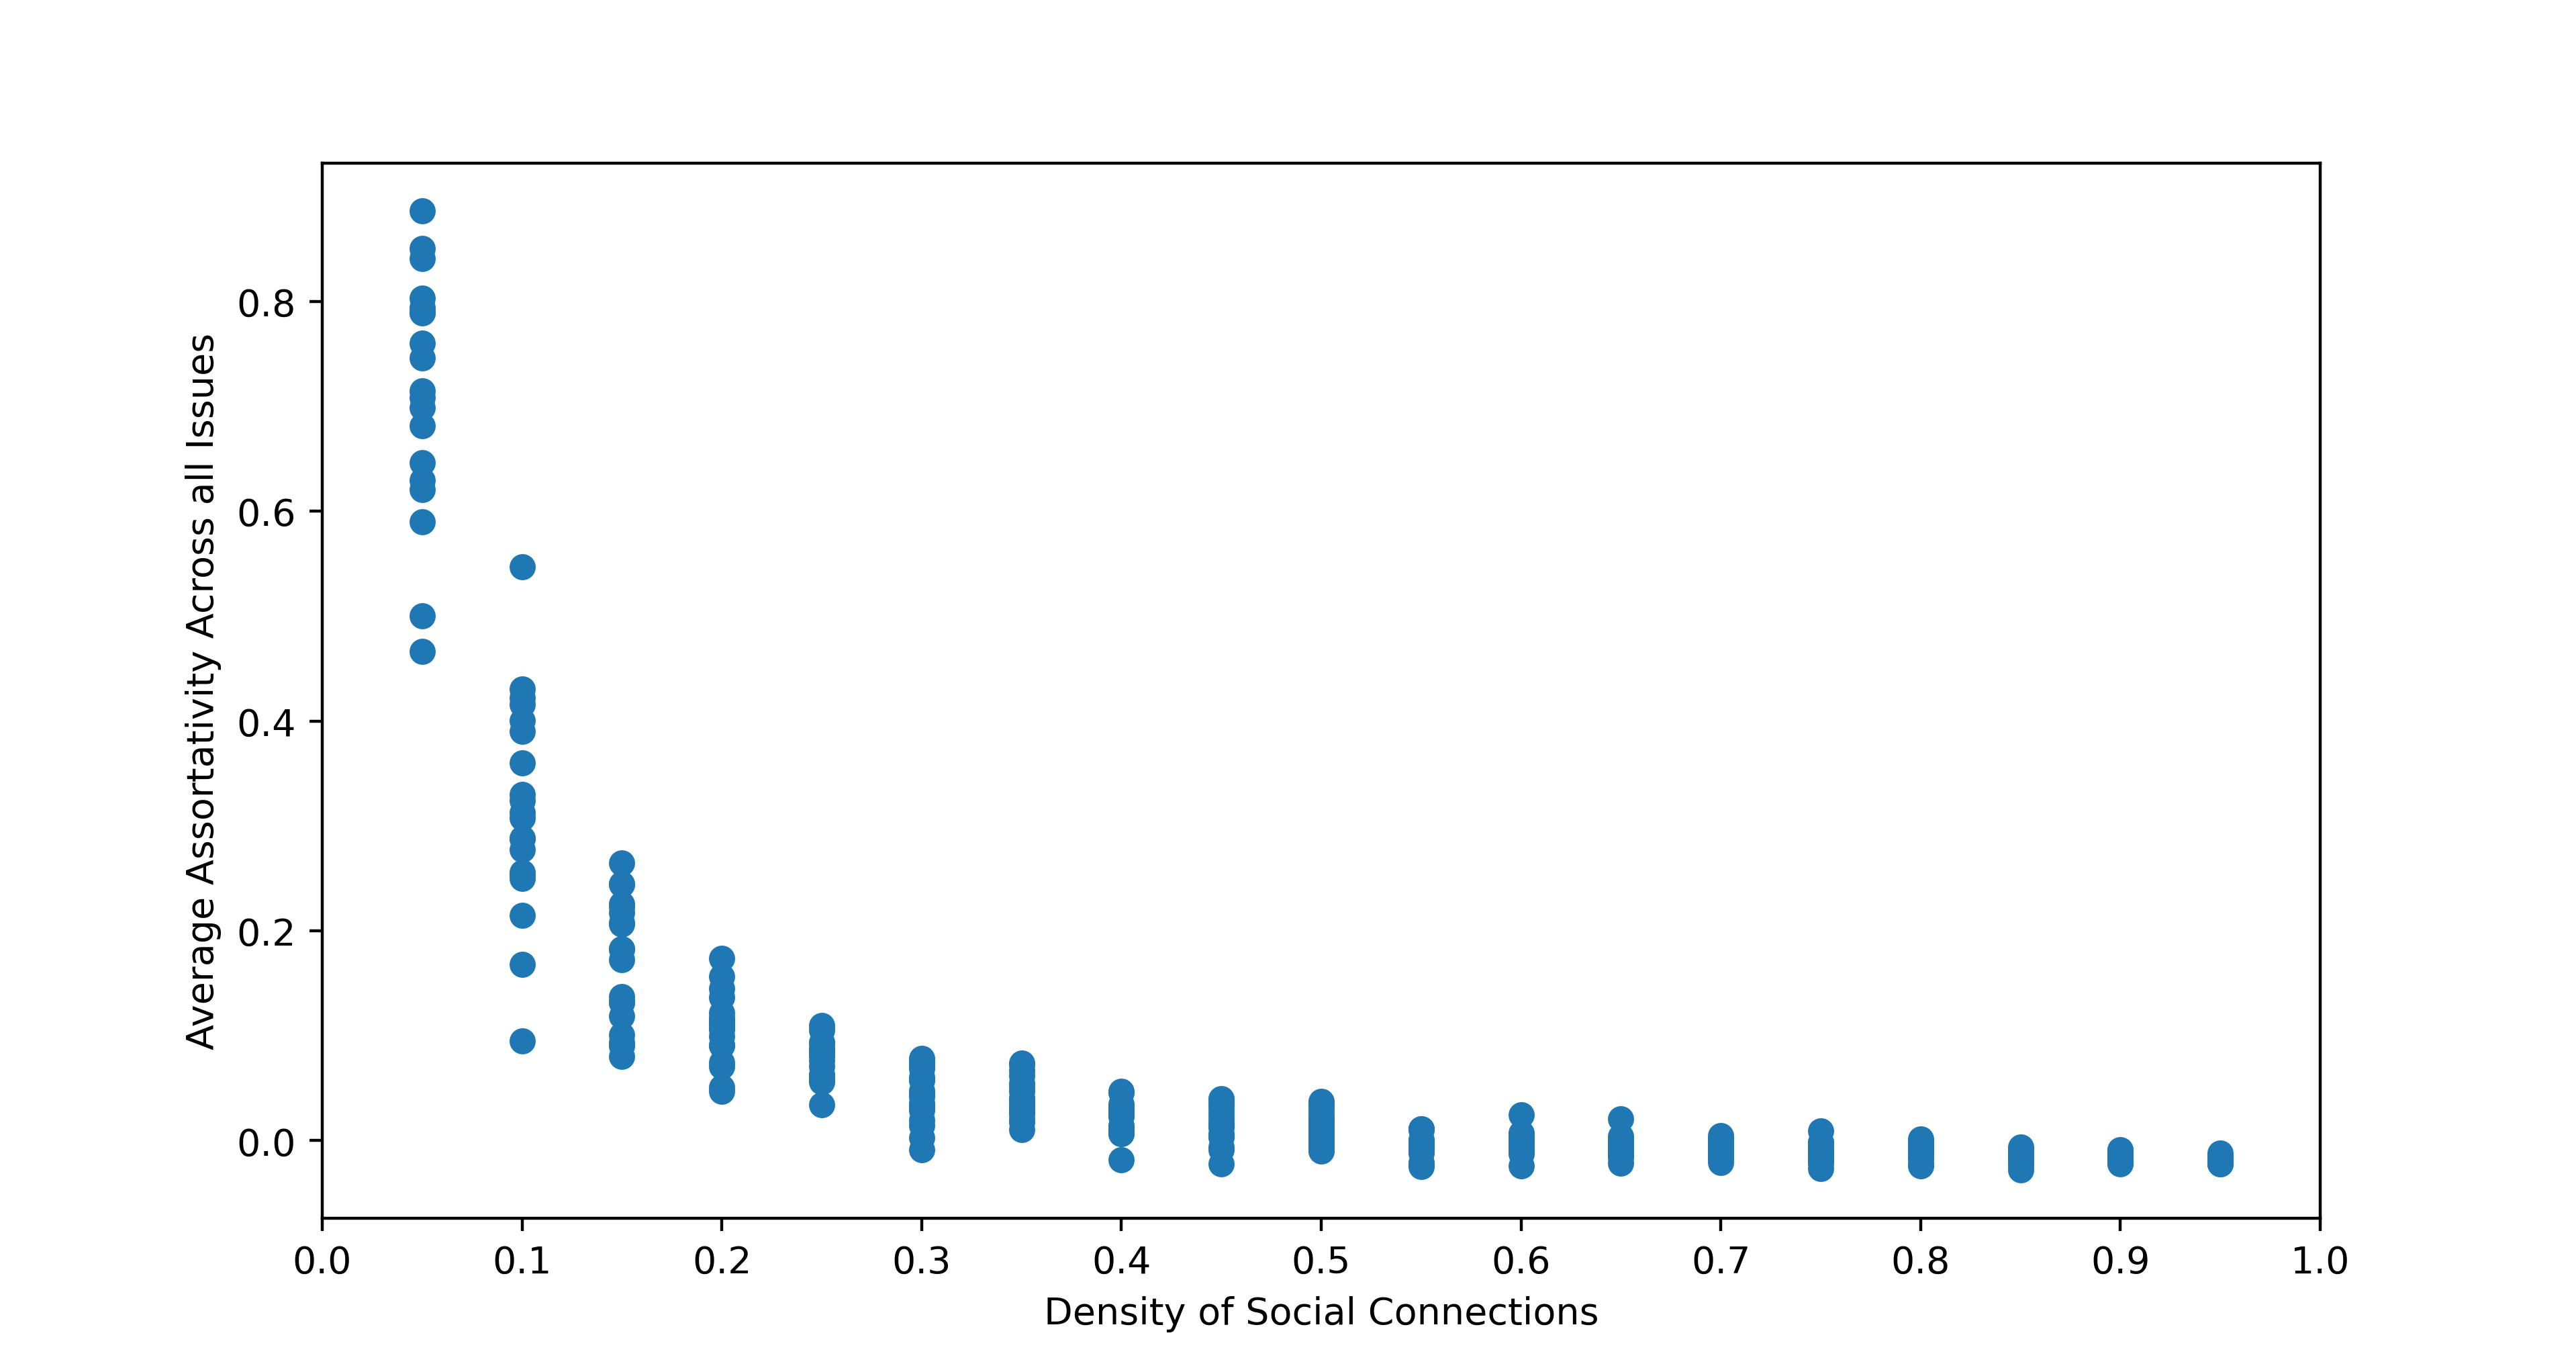
\includegraphics[width=0.9\textwidth]{images/Assort_edge.png}

\end{figure}

\vspace{-.3in}
\small
Fewer (meaningful) social connections = higher polarization BUT only at the low end.

\end{frame}

\begin{frame}[c]{Results: Assortativity and Agent Openness}  % Justin

% Walk them through what the axes are.
% Make the point that "if openness is zero, no one ever changes their mind, and
% so we would of course get zero assortativity (just random opinions)."
% 

% Higher openness can be viewed in two ways. It could mean "more open-minded
% and receptive to others' opinions." But it could also mean "more willing to
% blindly follow the opinions you hear around you." This latter interpretation
% is why we (paradoxically) see lower polarization for lower openness values.
% Takeaway: if a society's average openness is hovering between, say, .2 and
% .3, a little more critical thinking could move things left past the tipping
% point and end up with a less polarized society.

% TODO: Justin: put in a sentence here summarizing the findings you will
% articulate.

\begin{center}
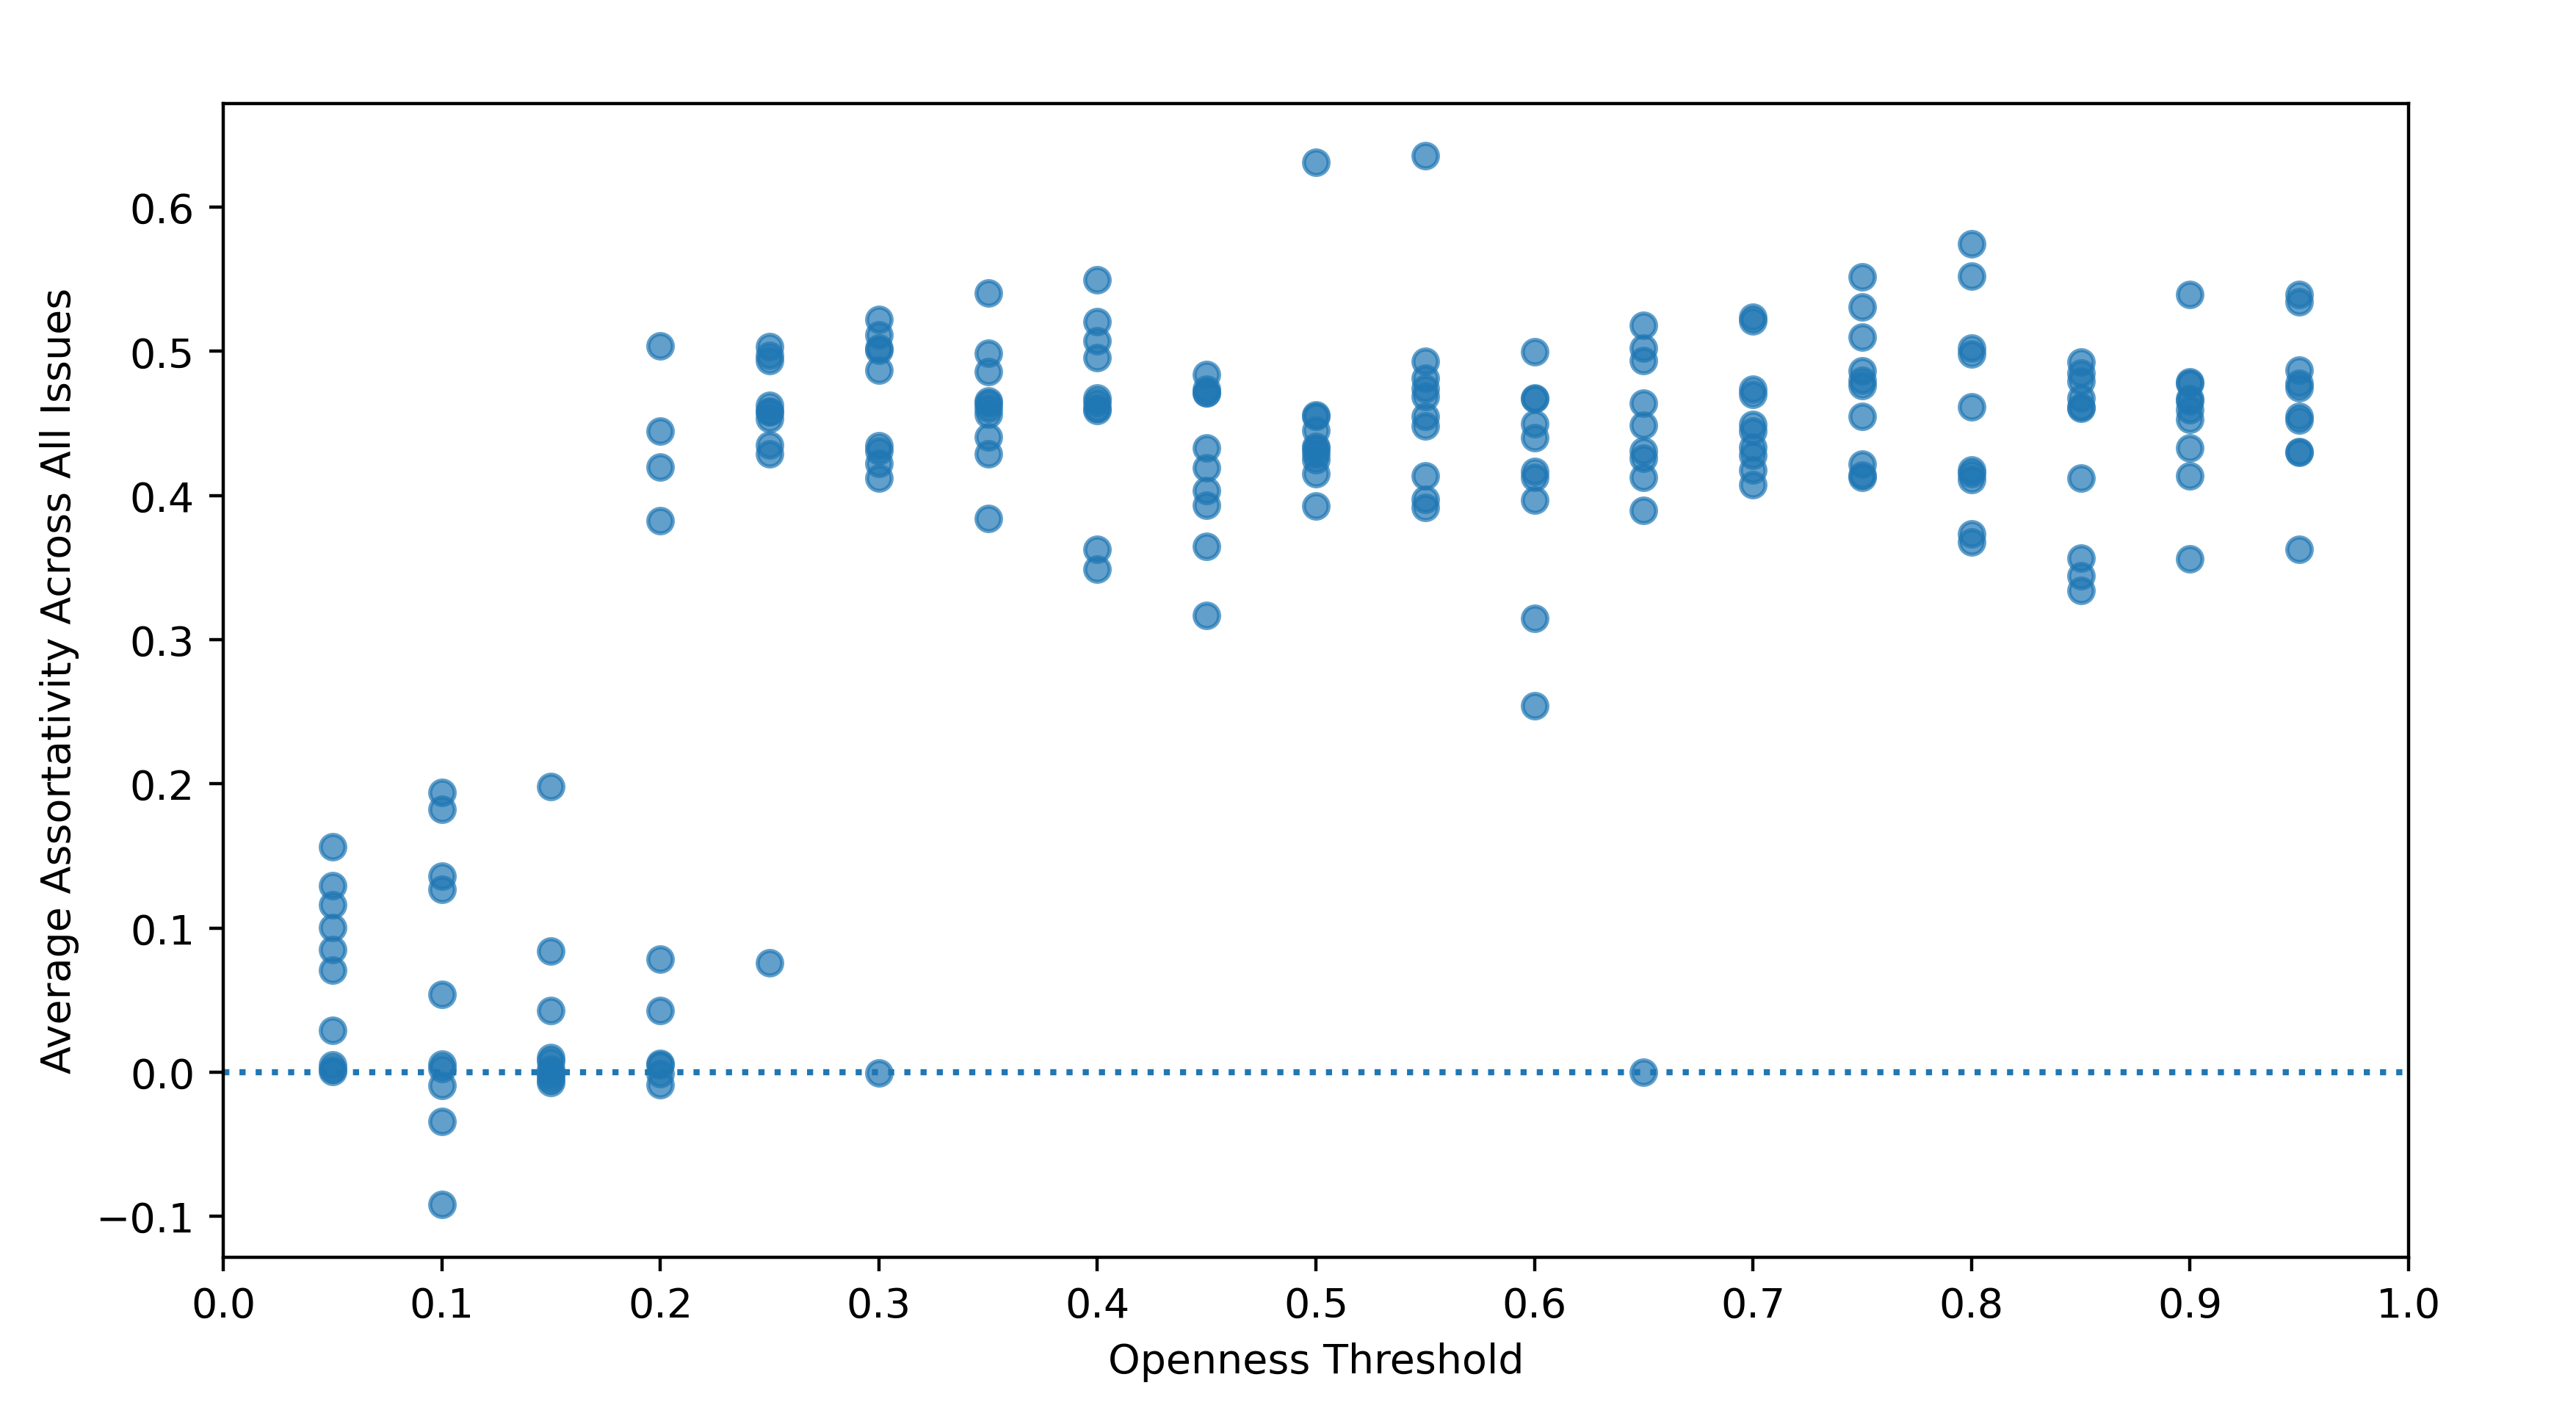
\includegraphics[width=0.9\textwidth]{images/AssortOpenness.png}
\small
Paradoxically, lower levels of openness \textit{decreased} polarization.
\end{center}

\end{frame}

\begin{frame}[c]{Polarization Proxy \#2: Issue Alignment} % Stephen

We define \textbf{Issue Alignment} (IA) as the tendency for people who agree on
one issue to also agree on other (unrelated) issues.

\begin{center}
\begin{tabular}{c|c}
\pause
raise the minimum wage & lower the minimum wage \\
\pause
pro-choice & pro-life \\
\pause
higher taxes \& services & lower taxes \& services \\
\pause
anti-guns & pro-guns \\
\pause
pro-immigration & anti-immigration \\
\pause
pro-vaccine-mandate & anti-vaccine-mandate \\
\pause
pro-renewable-energy & pro-fossil-fuels \\
\pause
... & ... \\
\end{tabular}
\end{center}

\pause
\footnotesize

If people generally adhere to an entire suite of opinions, we term that society
``Issue Aligned'' and claim this is an indication of polarization.

\end{frame}
\begin{frame}[c]{Issue Alignment (IA)} % Stephen

%\textbf{Issue Alignment} (IA): the tendency for people who agree on one issue
%to also agree on other (unrelated) issues.

\textit{Why} does IA occur?

Possible explanation \#1: perhaps there is some deep underlying
principle to people's value systems that connects seemingly unconnected issues.
\pause

\begin{center}
\begin{tabular}{clp{1cm}rc}
\makecell{
\\

\includegraphics[width=0.15\textwidth]{thinker1.jpg}
} &
\makecell{
Ideology 1 $\Rightarrow$ \\
Opinion A \\
Opinion B \\
Opinion C \\} & &
\makecell{
Ideology 2 $\Rightarrow$ \\
Opinion D \\
Opinion E \\
Opinion F \\} &
\makecell{
\\

\includegraphics[width=0.1\textwidth]{thinker2.jpg}
}
\end{tabular}
\end{center}

\end{frame}

\begin{frame}[c]{Issue Alignment (IA)} % Stephen

\textit{Why} does IA occur?

Possible explanation \#2: perhaps a small number of popular media
outlets each articulates a set of opinions on various issues. 

\pause
\begin{center}
\begin{tabular}{clp{1cm}rc}
\makecell{
\\

\includegraphics[width=0.15\textwidth]{listener1.jpg}
} &
\makecell{
News source 1:  \\
``Opinion A!'' \\
``Opinion B!'' \\
``Opinion C!'' \\} & &
\makecell{
News source 2:  \\
``Opinion D!'' \\
``Opinion E!'' \\
``Opinion F!'' \\} & 
\makecell{
\\

\includegraphics[width=0.15\textwidth]{listener2.jpg}
}
\end{tabular}
\end{center}

%The people who
%listen to them are naturally influenced to each of these different opinion
%values, and thus become ``issue aligned."

\end{frame}

\begin{frame}[c]{A third possible explanation for IA} % Stephen

\large
Our model demonstrates that neither ideological coherence nor media influence
is necessary for IA to develop. \textbf{Cross-issue influence} (CI2) is
sufficient.

\pause
\normalsize
\bigskip

This may have wide-reaching implications on how we interpret the causes of the
polarization phenomenon, and what societal changes might be necessary to reduce
it.

\end{frame}

\begin{frame}[c]{Cross-Issue Influence (Positive)}  % Stephen

We define \textbf{Cross-Issue Influence} (CI2) as the effect that an agent can
have on one of its neighbor's opinions based on their agreement (or
disagreement) on a \textit{different} issue. (Traditional BC models have used
``I2.'')

\pause
\begin{figure}
	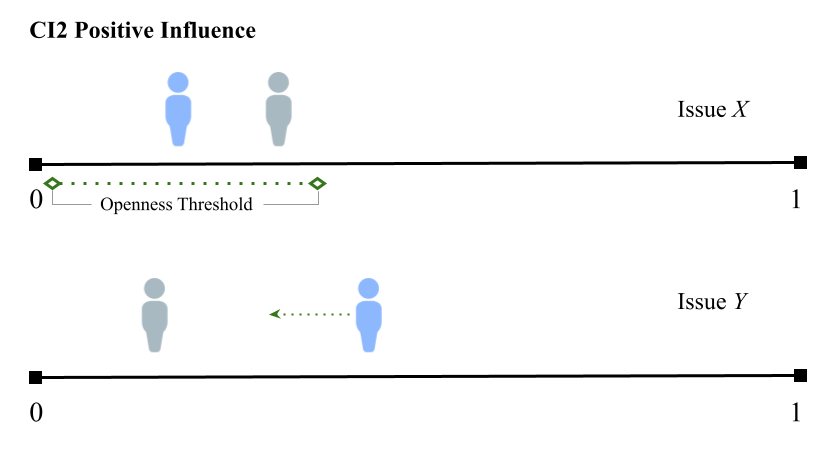
\includegraphics[width=0.75\textwidth]{images/CI2Positive.png}
	%TODO: add captions
\end{figure}

\end{frame}


\begin{frame}[c]{Cross-Issue Influence (Negative)}  % Stephen

% Show two number line and two peeps, with a repulsion due to disgust

% Also show the Justin threshold diagram with red & green regions

% And cite Griffin, Em (2011). A First Look at Communication Theory. New York,
% New York: McGraw Hill. pp. 194–204.
\begin{figure}
	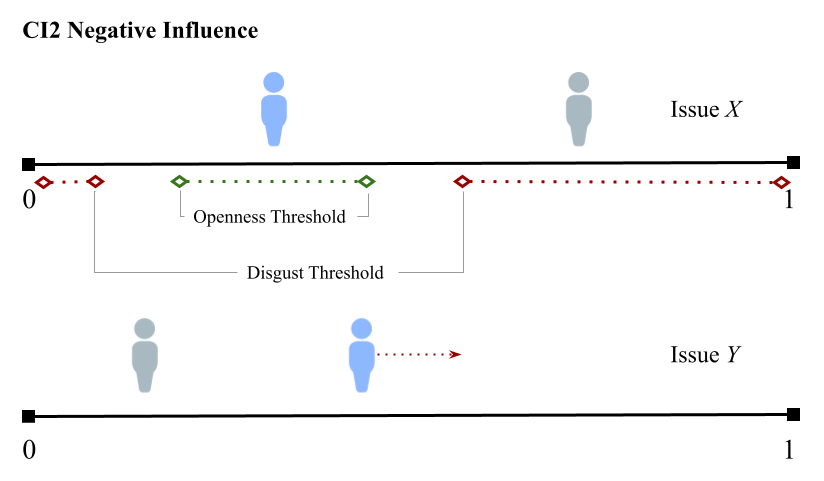
\includegraphics[width=0.75\textwidth]{images/CI2Negative.png}
\end{figure}

\end{frame}
\begin{frame}[c]{Quantifying IA} % Stephen

To measure the degree of Issue Alignment in a virtual society, we measure the
number of distinct opinion \textbf{buckets} that exist.

\bigskip
\pause
\begin{itemize}
\itemsep.1em

\item A ``bucket'' is a specific set of numerical opinions on the various issues.
\begin{itemize}
\itemsep.1em
\item For example: ``issue 1: \textbf{0.4}, issue 2: \textbf{1.0}, issue 3: \textbf{1.0}.''
\end{itemize}

\pause

\item At any point in simulated time, each agent is in one bucket, possibly with
other agents.

\pause
\item \textit{All agents in the same bucket agree on all the issues}, within a
threshold of $\varepsilon$ (.05).

\end{itemize}
\end{frame}


\begin{frame}[c]{Example} % Stephen

\begin{center}
\begin{tabular}{cp{1cm}c}
\makecell{
\small Agent $\alpha$: \\
\footnotesize Opinion on issue 1: \textbf{1.0} \\
\footnotesize Opinion on issue 2: \textbf{0.5} \\
\footnotesize Opinion on issue 3: \textbf{0.0} \\
} & &
\makecell{
\small Agent $\beta$: \\
\footnotesize Opinion on issue 1: \textbf{1.0} \\
\footnotesize Opinion on issue 2: \textbf{1.0} \\
\footnotesize Opinion on issue 3: \textbf{1.0} \\
} \\
\smallskip \\
\makecell{
\small Agent $\gamma$: \\
\footnotesize Opinion on issue 1: \textbf{0.6} \\
\footnotesize Opinion on issue 2: \textbf{0.0} \\
\footnotesize Opinion on issue 3: \textbf{0.2} \\
} & &
\makecell{
\small Agent $\delta$: \\
\footnotesize Opinion on issue 1: \textbf{1.0} \\
\footnotesize Opinion on issue 2: \textbf{0.5} \\
\footnotesize Opinion on issue 3: \textbf{0.0} \\
} \\
\end{tabular}

\bigskip
\bigskip
\smallskip
\phantom{In this model, there are \textbf{three} buckets: one with agents
$\alpha$ and $\delta$, one with agent $\beta$ only, and one with agent $\gamma$
only.}
\end{center}
\end{frame}

\begin{frame}[c]{Example} % Stephen

\begin{center}
\begin{tabular}{cp{1cm}c}
\makecell{
\color{darkgreen} \small Agent $\alpha$: \\
\color{darkgreen} \footnotesize Opinion on issue 1: \textbf{1.0} \\
\color{darkgreen} \footnotesize Opinion on issue 2: \textbf{0.5} \\
\color{darkgreen} \footnotesize Opinion on issue 3: \textbf{0.0} \\
} & &
\makecell{
\color{red} \small Agent $\beta$: \\
\color{red} \footnotesize Opinion on issue 1: \textbf{1.0} \\
\color{red} \footnotesize Opinion on issue 2: \textbf{1.0} \\
\color{red} \footnotesize Opinion on issue 3: \textbf{1.0} \\
} \\
\smallskip \\
\makecell{
\color{blue} \small Agent $\gamma$: \\
\color{blue} \footnotesize Opinion on issue 1: \textbf{0.6} \\
\color{blue} \footnotesize Opinion on issue 2: \textbf{0.0} \\
\color{blue} \footnotesize Opinion on issue 3: \textbf{0.2} \\
} & &
\makecell{
\color{darkgreen} \small Agent $\delta$: \\
\color{darkgreen} \footnotesize Opinion on issue 1: \textbf{1.0} \\
\color{darkgreen} \footnotesize Opinion on issue 2: \textbf{0.5} \\
\color{darkgreen} \footnotesize Opinion on issue 3: \textbf{0.0} \\
} \\
\end{tabular}

\bigskip
{In this model, there are \textbf{three} buckets: one with agents
$\alpha$ and $\delta$, one with agent $\beta$ only, and one with agent $\gamma$
only.}
\end{center}
\end{frame}


\begin{frame}[c]{Interpretation} % Stephen

\large
We interpret \textbf{fewer buckets} to mean \textbf{more Issue Alignment} (and hence, more polarization).

\pause
\normalsize
\bigskip
One other bit of lingo:

\begin{itemize}
\itemsep.1em
\item If a pair of agents agrees on \textit{every} issue (\textit{i.e.}, they're in
the same bucket), we call them \textbf{clones} (or a ``clone pair.'')

\bigskip

\item If a pair of agents \underline{dis}agrees on every issue, we call them
\textbf{anti-clones} (or an ``anti-clone pair.'')
\end{itemize}

\end{frame}


\begin{frame}[c]{Census plot: number of agreements (\textbf{I2 only})} % Stephen

\vspace{-.3in}
\begin{center}
\hspace{-.6in} 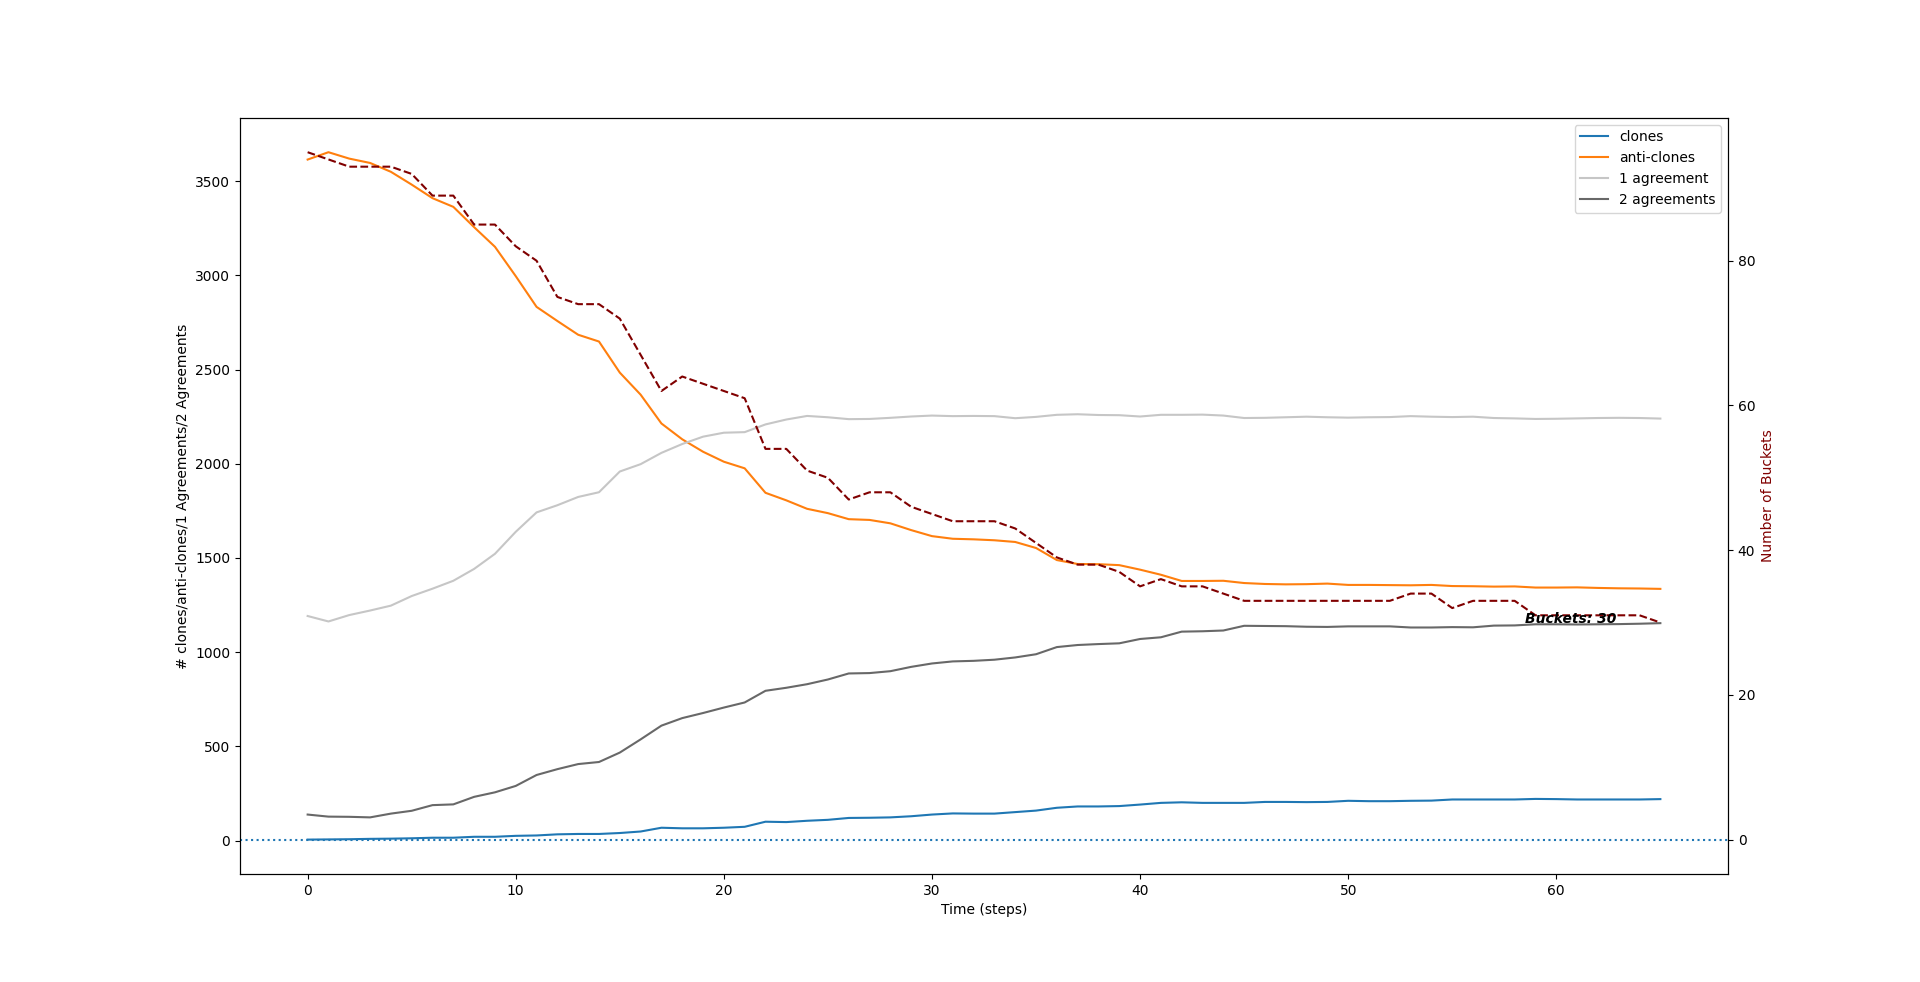
\includegraphics[width=1.11\textwidth]{census3issuesI2.png}
\vspace{-.3in}
\scriptsize (Three issues)
\end{center}

\end{frame}

\begin{frame}[c]{Census plot: number of agreements (\textbf{with CI2})} % Stephen

\vspace{-.3in}
\begin{center}
\hspace{-.6in} 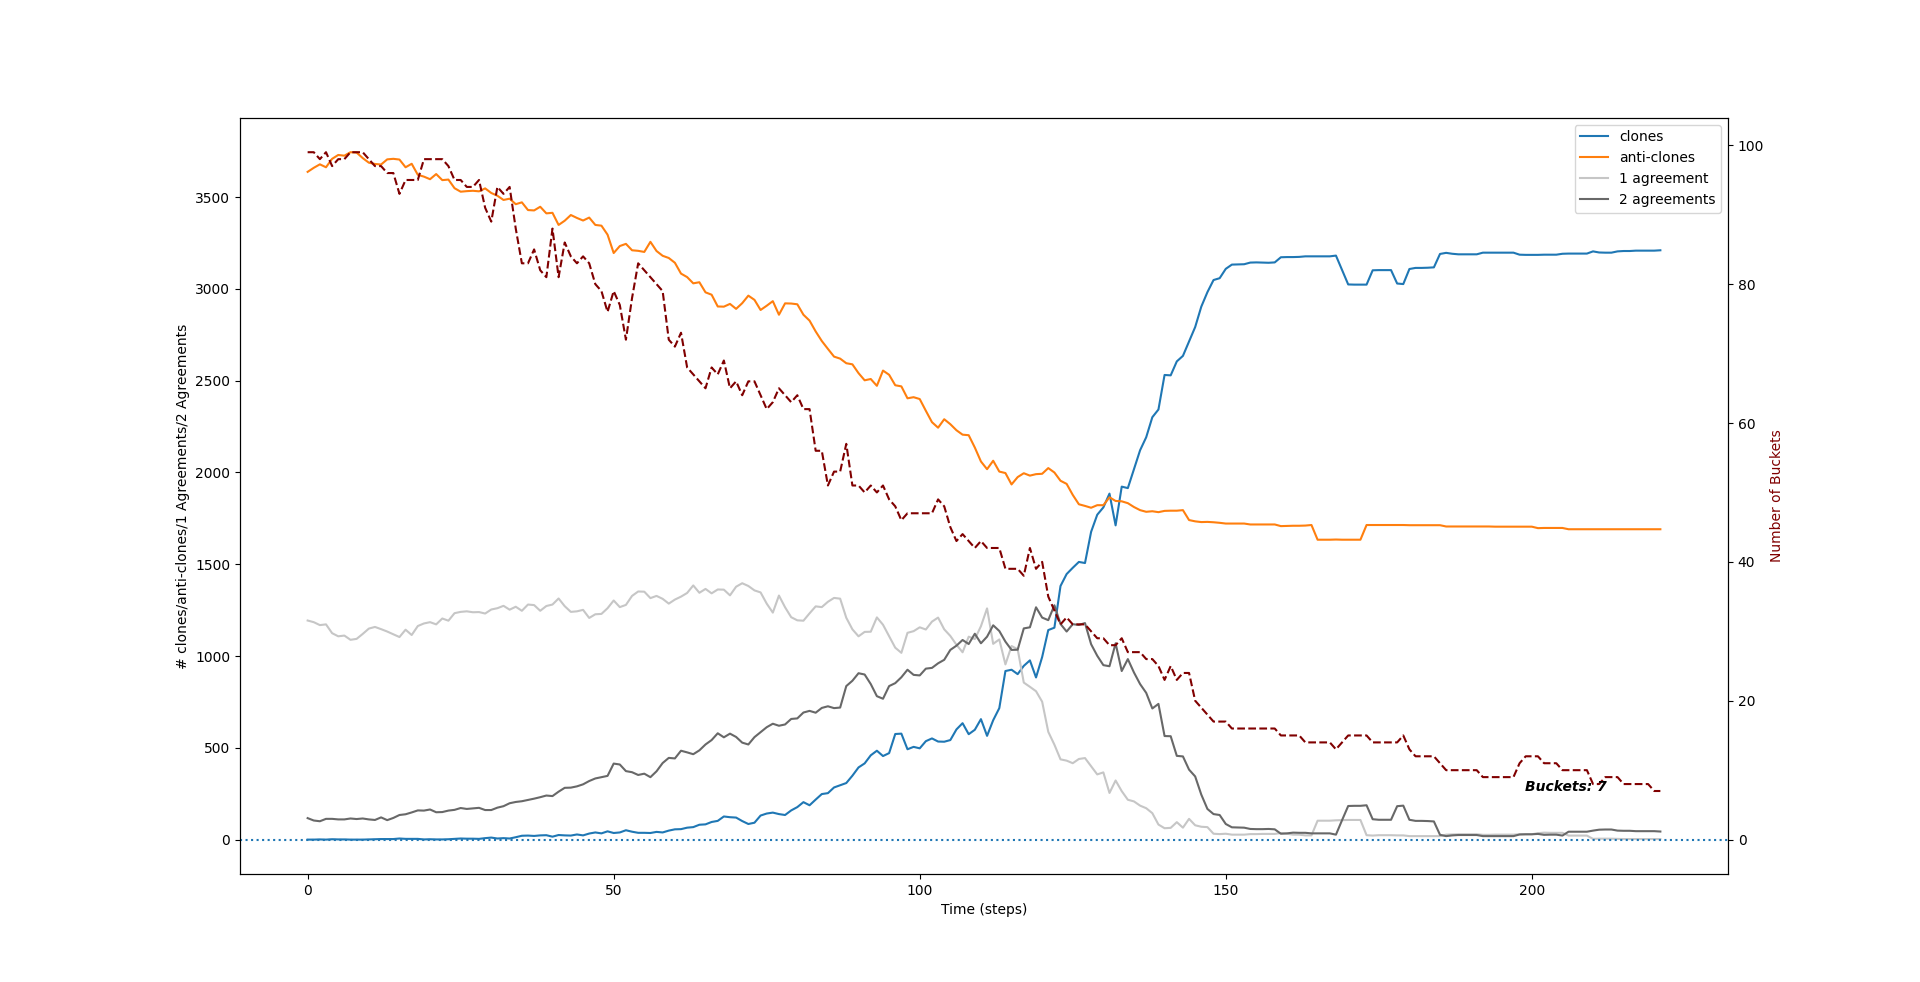
\includegraphics[width=1.11\textwidth]{census3issuesCI2.png}
\vspace{-.3in}
\scriptsize (Three issues)
\end{center}

\end{frame}

\begin{frame}[c]{Census plot: number of agreements (\textbf{with CI2})} % Stephen

\vspace{-.3in}
\begin{center}
\hspace{-.6in} 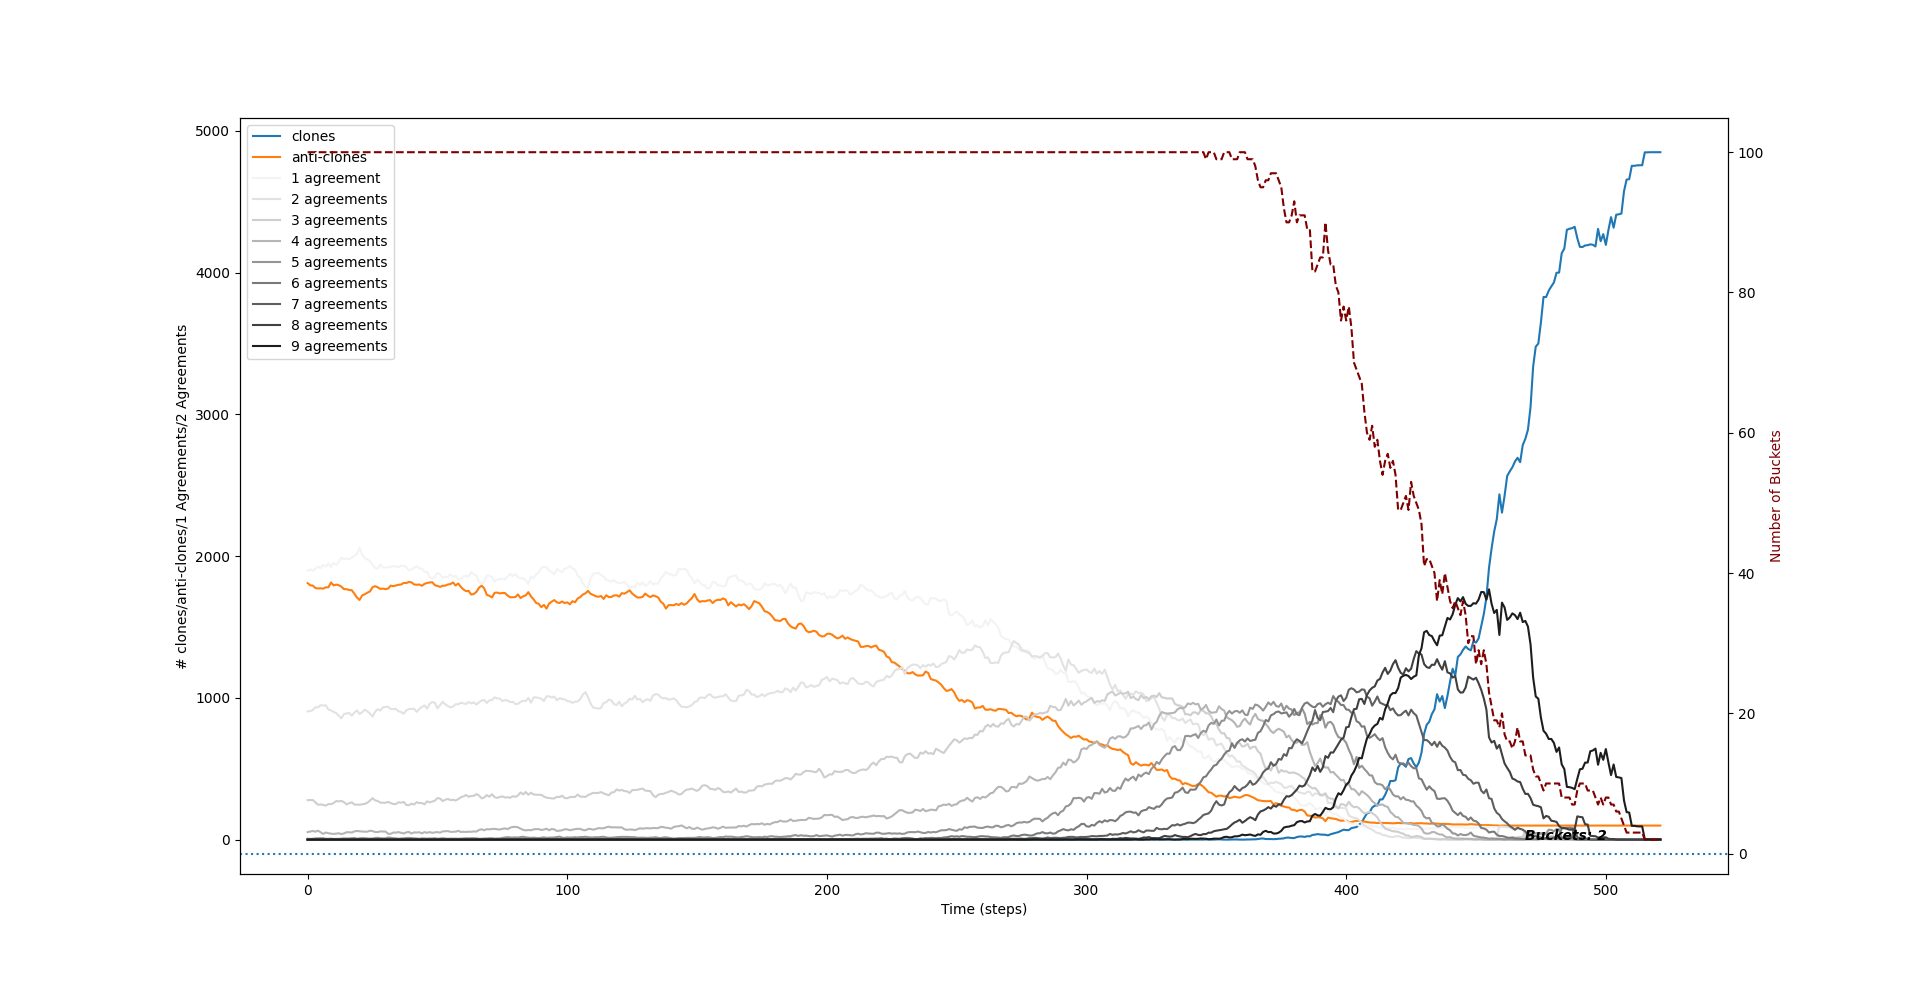
\includegraphics[width=1.11\textwidth]{census10issuesCI2.png}
\vspace{-.3in}
\scriptsize (Ten issues)
\end{center}

\end{frame}

%\begin{frame}[c]{Heat maps: showing interplay of openness and disgust threshold
%with and without CI2} % Stephen
%
%\end{frame}


% Tuck-away slide
%\begin{frame}[c]{Diametricity}
%
%One other way to define polarization is extremity of views.
%
%Fact: if CI2 is employed, the model always (?) produces exactly two buckets,
%and all the opinions in those buckets are at the poles.
%
%Fact: if only I2 is employed, there will normally be many buckets (often one
%for each combination of fully-polarized opinions; i.e., a (0,0,0) bucket, a
%(0,0,1), (0,0,2), (0,1,0), ...)
%
%\end{frame}

\begin{frame}[c]{Discussion and takeaways}  % Stephen & Justin

%Justin:
Lower network density leads to higher polarization. Takeaway: people need to
get out more.

%(If you are hearing from more individuals, you will be likely to
%hear a more diverse set of opinions and won't get in an echo chamber as
%easily.)

\pause
%Justin:
If people are ``too open'' and easily believe what they hear, this can lead to
echo chambers forming more readily. Takeaway: be more cautious and discerning
about what you hear.
% could mention "openness is a double-edged sword. On the one hand, you want to
% be open to others' viewpoints. On the other hand, if you're too gullible, it
% can make echo chambers happen more readily."

\pause
% Stephen:
IA endogenously appears with CI2. We can't solely blame media outlets or
ideologies.

\pause
Individual fix: Allow yourself the freedom to agree with someone on one thing
and disagree with them on something else.

\pause
Society's fix: parties and global media outlets undoubtedly reinforce the IA
phenomenon. We need voices from more buckets!

\end{frame}

\begin{frame}[c]{}

\begin{center}
\Large
The Impact of Social Network Density,\\Agent Openness, and Cross-Issue
Influence\\on Societal Polarization

\footnotesize
\vspace{.3in}
CSS 2021 --- Santa Fe, New Mexico (sorta)\\
\vspace{.1in}
\textbf{Justin Mittereder}, Robert Carroll, Brandon Frulla,
\textbf{Stephen Davies}\\
\scriptsize
\smallskip
Dept of Computer Science\\
University of Mary Washington\\
Fredericksburg, Virginia, USA\\
\bigskip
\bigskip
\texttt{https://github.com/jmittere/Peacemakers}
\end{center}

\end{frame}
\end{document}


% Point #1 (in this prez): CI2 results in fewer buckets (histogram showing # of
% buckets for both I2 and CI2)
% Point #2 (for later): interplay between openness and disgust (heatmap showing 
% openness vs disgust vs # of buckets. Probably don't need to show both I2 and
% CI2 heatmaps because they tell the same story.)
